\documentclass[pdftex,12pt,a4paper]{article}

\usepackage{amssymb}
\usepackage[pdftex]{graphicx}
\usepackage{etoolbox}
\usepackage{paralist}
\usepackage{mathtools}
\usepackage{hyperref}
\usepackage{floatflt}
\usepackage[xindy]{glossaries}
\usepackage[utf8]{inputenc}
\usepackage[ngerman]{babel}
\usepackage{bookmark}
\usepackage{fancyhdr}
\usepackage{lastpage}
\usepackage[style=authoryear,backend=biber]{biblatex}
\addbibresource{./bibliography.bib}
\usepackage[ngerman]{babel}
\usepackage[babel,german=quotes]{csquotes}
\usepackage[font=footnotesize,labelfont=bf]{caption}

% Set TOC title
\renewcommand{\contentsname}{Inhalt}
\addto\captionsngerman{\renewcommand{\contentsname}{Inhalt}}
\pagestyle{fancy}
\fancyhf{}
\fancyhead[L]{\rotatebox{0}{\scalebox{0.5}[0.5]{
\includegraphics{images/BFH_Logo_C_de_100_RGB.png}}}}
\fancyhead[C]{}
\fancyhead[R]{}
\renewcommand{\headrulewidth}{0.4pt}
\fancyfoot[R]{\thepage /  \pageref{LastPage}}
\renewcommand{\footrulewidth}{0.4pt}

\newcommand{\HRule}{\rule{\linewidth}{0.5mm}}

\newglossaryentry{tesselation}{name=Tesselation,
    description={zu Deutsch Parkettierung. Frei übersetzt nach \citeauthor{schwartzman1994words}. `Von dem lateinischen Wort \textit{tessera} ``eine viereckige Tafel'' oder ``ein Würfel, benutzt zum Spielen''. Das lat. Wort \textit{tessera} wurde sehr wahrscheinlich von dem griechischen Wort tessares, was soviel wie ``vier'' bedeutet, abgeleitet bzw.\ ausgeliehen, da ein quadratisches Feld über vier Seiten verfügt. Die Kurzform von tessera war \textbf{tessella}, ein kleines, quadratisches Stück Stein oder eine kubische Kachel, wie sie bei Mosaik zur Verwendung kommt. Da ein Mosaik sich über eine gegebene Fläche ersttreckt, ohne eine Region auszulassen, ist die geometrische Bedeutung des Wortes tessellieren ``eine Ebene mit einem Muster bedecken, so dass keine Region unbedeckt bleibt.''. Raum oder Hyperraum kann auch tesseliert werden (\citeyear{schwartzman1994words})}
}

\newglossaryentry{dualGraph}{name=Dualer Graph,
    description={Gegeben sei $G$, ein kreuzungsfreier, nicht leerer und zusammenhängender Graph. Wie~\cite{klein2005algorithmischegeometrie} angibt, ist ein Graph $G*$ dann dual zu $G$, wenn Folgendes gilt:
    \begin{compactitem}
    \item Im Innern jeder Fläche von $G$ werden neue Punkte $p_F^*$ hinzugefügt. Dies sind die Knoten von $G^*$.
    \item Für jede Kante $e$ (edge) von $G$, welche die angrenzenden Flächen $F$ und $F'$ besitzt, werden die Punkte $p_F^*$ und $p_{F'}^*$ zu einer Kante $e^*$ verbunden. Diese kreuzt nur die Kante $e$ und sonst keine andere Kante.
    \end{compactitem}
    Wenn dies gilt, dann ist $\boldsymbol{G^*}$ der \textbf{\textit{duale Graph}} von $G$. ${(G^*)}^*$ ist wiederum zum Graphen $G$ äquivalent}
}


\newglossaryentry{bigOh}{name=Gross-Oh $O()$,
    description={Die Gross-Oh-Notation $O$ besagt, dass eine Funktion maximal das asymptotische Wachstumsverhalten der angegebenen Funktion aufweist, beispielsweise:
\noindent\hspace*{10mm}%
$g \in O(f)$
Dies besagt, dass die Funktion $g$ in ihrem asymptotischen Wachstum praktisch überall (bis auf einen konstanten Faktor) durch die Funktion $f$ beschränkt ist.
Sie bildet also eine Art obere Schranke. Frei nach~\citeauthor{goodrich2002algorithm} übersetzt (\citeyear[S. 13]{goodrich2002algorithm})}
}

\newglossaryentry{bigOmega}{name=Gross-Omega $\Omega()$,
    description={Die Gross-Omega-Notation $\Omega$ definiert eine untere Schranke, welche besagt, dass eine Funktion bis auf einen konstanten Faktor in ihrem asymptotischen Wachstum grösser oder gleich einer anderen Funktion ist,
beispielsweise:
\noindent\hspace*{10mm}%
$g \in \Omega(f)$
Wodurch auch $f \in O(g)$ gilt. Frei nach~\citeauthor{goodrich2002algorithm} übersetzt (\citeyear[S. 16 bis 17]{goodrich2002algorithm})}
}

\newglossaryentry{bigTheta}{name=Gross-Theta $\Theta()$,
    description={Die Gross-Theta-Notation $\Theta$ erlaubt es, zu sagen, dass zwei Funktionen $g$ und $f$ bis zu einem konstanten Faktor dasselbe asymptotische Wachstumsverhalten aufweisen, beispielsweise:
\noindent\hspace*{10mm}%
$g \in \Theta(f)$
Wodurch auch $g \in O(f)$ und $g \in \Omega(f)$ gilt. Frei nach~\citeauthor{goodrich2002algorithm} übersetzt (\citeyear[S. 16 bis 17]{goodrich2002algorithm})}
}

\newglossaryentry{simplex}{name=Simplex,
  description={Eine konvexe Hülle von $n + 1$ Punkten im $\mathbb{R}^d$, $n <= d$, die nicht in einem $(n - 1)$-dimensionalen Teilaraum liegen, nennt man das Simplex der Dimension $n$~\parencite[S. 23]{klein2005algorithmischegeometrie}}
}

\newglossaryentry{bisector}{name=Bisektor,
  description={Eine Gerade zwischen zwei Punkten, bestehend aus Punkten, welche genau denselben Abstand zu den zwei Punkten haben~\parencite[S. 25]{klein2005algorithmischegeometrie}}
}

\newglossaryentry{euclideanDistance}{name=Euklidischer Abstand,
  description={Bestimmt den Abstand zweier Punkte. $|x_i - x_j| = \sqrt{{\sum_{k=1}^{m} {(x_ik - x_jk)}^2}}$~\parencite[S. 16]{atsuyuki2000spatialtessellations}}
}

\newglossaryentry{convexHull}{name=Konvexe Hülle,
  description={Informell gesagt handelt es sich dabei um die Hülle eines Gummibandes, welches um eine Punktemenge in der Ebene gelegt wird. Oder, etwas formeller: ``Eine Region $R$ ist \textbf{konvex}, wenn jederzeit gilt, dass sich zwei Punkte $p$ und $q$, sowie deren Liniensegment $\overline{pq}$ in $R$ befinden. Die \textbf{konvexe Hülle} einer Punktemenge $S$ ist der Umfang der schmalsten konvexen Region, welche alle Punkte von $S$ beinhaltet bzw\. auf deren Rand hat.''. Frei nach~\citeauthor{goodrich2002algorithm} übersetzt (\citeyear[S. 572 bis 576]{goodrich2002algorithm})}
}

\makeglossaries
% Add all glossary entries no matter if they get
% referenced or not
\glsaddall

\setlength{\headheight}{32pt}
\setlength{\abovecaptionskip}{2pt plus 3pt minus 2pt}
\setlength{\parindent}{0pt}
\setlength{\parskip}{10pt plus 1pt minus 1pt}

\apptocmd{\sloppy}{\hbadness 10000\relax}{}{}

% Add all bibliography entries no matter if they
% get cited or nod
\nocite{*}

\begin{document}

%deckblatt start
\thispagestyle{empty}
\begin{center}
\rotatebox{0}{\scalebox{1.0}[1.0]{
\includegraphics{images/BFH_Logo_C_de_100_RGB.png}}}\\
\end{center}
\begin{center}
\Large{Berner Fachhochschule (BFH)}\\
\end{center}
 
 
\begin{center}
\Large{Departement Informatik}
\end{center}
\begin{verbatim}
\end{verbatim}
\begin{center}
\textbf{\LARGE{BTI7311 - Informatik Seminar}}
\end{center}
\begin{verbatim}
 
 
\end{verbatim}
\begin{center}
\textbf{Bericht}
\end{center}
\begin{verbatim} 
\end{verbatim}
 
\begin{flushleft}
\begin{tabular}{lll}
\textbf{Thema:} & & Voronoidiagramme und Delaunay-Triangulation\\
& & \\
& & \\
& & \\
\textbf{Student:} & & Sven Osterwalder (ostes2@bfh.ch)\\
& & \\
& & \\
\textbf{Date:} & & {\today}\\
& & \\
& & \\
\textbf{Professor:} & & Prof. Pierre Fierz
\end{tabular}
\end{flushleft}

\newpage

\tableofcontents

\newpage

\subsection{Einführung}
\label{subsec:delaunay-introduction}

Wie in~\cite{atsuyuki2000spatialtessellations} angegeben, kann aus einem gegeben, $m$-dimensionalen Voronoi-Diagramm ein weiteres, zum Voronoi-Diagramm duales Diagramm abgeleitet werden. Es handelt sich dabei um die Delaunay-Tesselation bzw. -Triangulation. Dabei werden die Punkte, deren Regionen eine $(m-1)$-dimensionale Oberfläche teilen, verbunden.

Die Delaunay-Tesselation kann allerdings auch direkt aus der Punktemenge erstellt werden, indem jeweils der Umkreis von $(m+1)$ Punkten betrachtet wird. Befindet sich keiner der Puntke aus der Menge in der Fläche des Kreises, wird ein Simplex aus den $(m+1)$ Punkten gebildet. Befindet sich ein Punkt in der Fläche, wird nichts unternommen. Dies geschieht so lange, bis alle möglichen Flächen über $(m+1)$ Punkte gebildet wurden.

\begin{figure}[h]
\centering
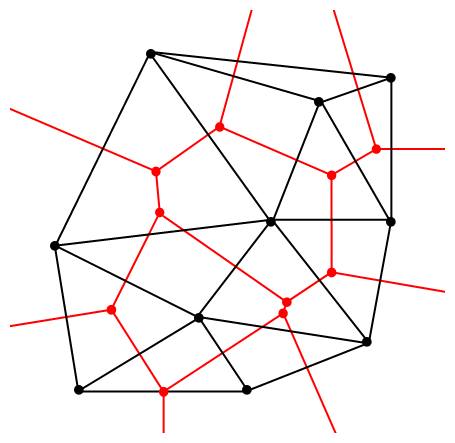
\includegraphics[width=130px]{images/voronoi_delaunay_example_01.png}
\caption{Beispiel einer Delaunay-Triangulation (schwarz) anhand eines Voronoidiagramms (rot)}
\label{fig:delaunayVoronoiExample}
\end{figure}


In der Computergrafik werden in der Regel Polygone verwendet um 2D- oder auch 3D-Modelle darzustellen, sprich, zu rendern. Um diese Modelle möglichst schnell und effizient darzustellen wird bei den Grafikkarten stark auf Optimierung gesetzt. So wird eine Fläche, welche aus Dreiecken besteht, sehr effizient dargestellt. Dies, da ein Dreieck aus drei Punkten besteht und alle diese Punkte auf der selben Ebene liegen, was den Vorgang der Rasterisierung (vereinfacht, die Darstellung einer n-dimensionalen Szene auf einer zweidimensionalen Fläche) deutlich vereinfacht.

Die Delaunay-Triangulation ermöglicht es auf eine effiziente Weise beliebige Flächen zu triangulieren. Wie bereits in~\ref{sec:introduction} erwähnt, kann dies beispielsweise dazu genutzt werden um eine Oberfläche in einem Geoinformationssystem oder ein Polygonnetz zur Darstellung eines dreidimensionalen Modells in einer in Echtzeit auf digitaler Hardware erzeugten multimedialen Präsentation zu erzeugen.

\begin{figure}[h]
\centering
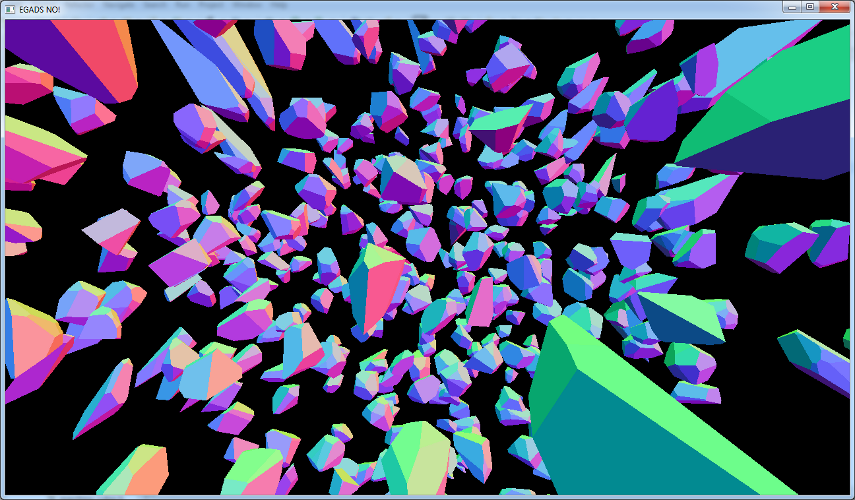
\includegraphics[width=200px]{images/voronoi_delaunay_example_02.png}
\caption[width=100px]{Beispiel von Polygon-Modellen, welche mit Delaunay-Triangulation erzeugt wurden}
\label{fig:delaunayVoronoiExample2}
\end{figure}


\section{Grundlagen}

[Beschreibung der Grundlagen. Was sind Voronoi-Diagramme, was ist die Delaunay-Triangulation?]


\section{Voronoi-Diagramme}

\subsection{Einführung}
\label{subsec:delaunay-introduction}

Wie in~\cite{atsuyuki2000spatialtessellations} angegeben, kann aus einem gegeben, $m$-dimensionalen Voronoi-Diagramm ein weiteres, zum Voronoi-Diagramm duales Diagramm abgeleitet werden. Es handelt sich dabei um die Delaunay-Tesselation bzw. -Triangulation. Dabei werden die Punkte, deren Regionen eine $(m-1)$-dimensionale Oberfläche teilen, verbunden.

Die Delaunay-Tesselation kann allerdings auch direkt aus der Punktemenge erstellt werden, indem jeweils der Umkreis von $(m+1)$ Punkten betrachtet wird. Befindet sich keiner der Puntke aus der Menge in der Fläche des Kreises, wird ein Simplex aus den $(m+1)$ Punkten gebildet. Befindet sich ein Punkt in der Fläche, wird nichts unternommen. Dies geschieht so lange, bis alle möglichen Flächen über $(m+1)$ Punkte gebildet wurden.

\begin{figure}[h]
\centering
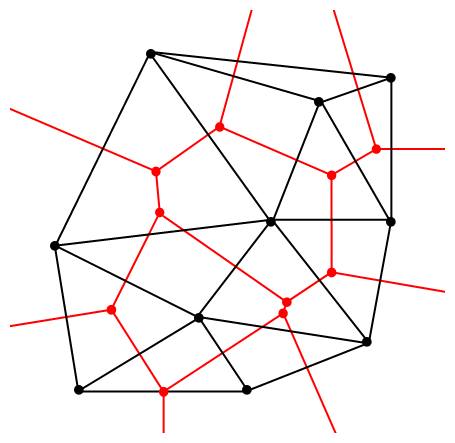
\includegraphics[width=130px]{images/voronoi_delaunay_example_01.png}
\caption{Beispiel einer Delaunay-Triangulation (schwarz) anhand eines Voronoidiagramms (rot)}
\label{fig:delaunayVoronoiExample}
\end{figure}


In der Computergrafik werden in der Regel Polygone verwendet um 2D- oder auch 3D-Modelle darzustellen, sprich, zu rendern. Um diese Modelle möglichst schnell und effizient darzustellen wird bei den Grafikkarten stark auf Optimierung gesetzt. So wird eine Fläche, welche aus Dreiecken besteht, sehr effizient dargestellt. Dies, da ein Dreieck aus drei Punkten besteht und alle diese Punkte auf der selben Ebene liegen, was den Vorgang der Rasterisierung (vereinfacht, die Darstellung einer n-dimensionalen Szene auf einer zweidimensionalen Fläche) deutlich vereinfacht.

Die Delaunay-Triangulation ermöglicht es auf eine effiziente Weise beliebige Flächen zu triangulieren. Wie bereits in~\ref{sec:introduction} erwähnt, kann dies beispielsweise dazu genutzt werden um eine Oberfläche in einem Geoinformationssystem oder ein Polygonnetz zur Darstellung eines dreidimensionalen Modells in einer in Echtzeit auf digitaler Hardware erzeugten multimedialen Präsentation zu erzeugen.

\begin{figure}[h]
\centering
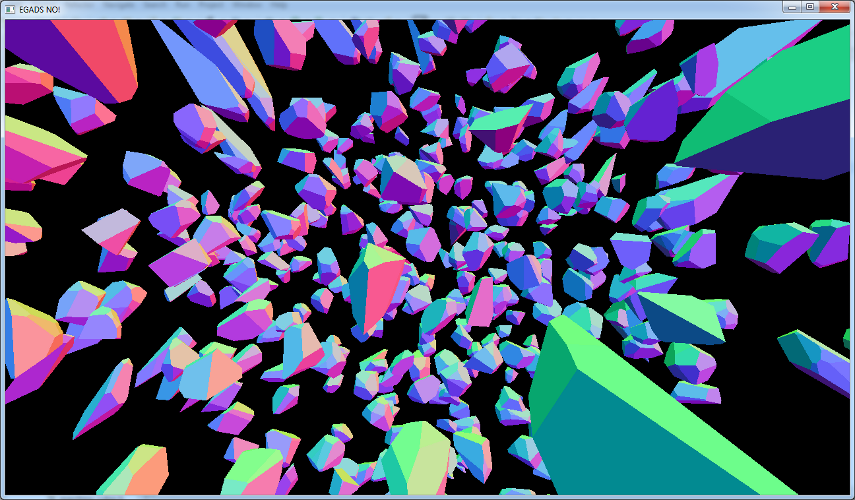
\includegraphics[width=200px]{images/voronoi_delaunay_example_02.png}
\caption[width=100px]{Beispiel von Polygon-Modellen, welche mit Delaunay-Triangulation erzeugt wurden}
\label{fig:delaunayVoronoiExample2}
\end{figure}


\subsection{Definition und Struktur}

Der Einfachheit halber wird in diesem Abschnitt der Raum $\mathbb{R}^2$ anstatt der unter ~\ref{subsec:voronoi-introduction} eingeführte Raum $\mathbb{R}^m$ verwendet.

Die Voronoi-Region $VR(p, O)$ besteht aus allen Punkten der Ebene, denen der Punkt $p = {p_x, p_y}$ näher ist als jeder andere Punkt aus der Punktemenge $O$.

Entfernt man nun sämtliche Voronoi-Regionen aus der Ebene, bleiben genau die Punkte des Raumes $\mathbb{R}^2$ übrig, die keinen eindeutigen sondern zwei oder mehr nächste Nachbaren in der Objekt-Menge $O$ besitzen.

Diese Punktemenge ist das \textit{Voronoi-Diagramm} $V(O)$ von $O$. \parencite{klein2005algorithmischegeometrie}


\subsection{Algorithmen}
Vorstellung von versch. Algorithmen für Voronoi-Diagramme (sofern mehrere existieren), Laufzeitverhalten, Komplexität, Vor- und Nachteile.]

\subsection{Verallgemeinerte Form}
[Beschreibung der verallgemeinerten Form von Voronoi-Diagrammen.]

\subsection{Praktische Anwendung}
[Ausblick auf praktische Anwendungen und Implementationen, ggf. eigene Implementation.]

\newpage
\section{Delaunay-Triangulation}

\subsection{Einführung}
\label{subsec:delaunay-introduction}

Wie in~\cite{atsuyuki2000spatialtessellations} angegeben, kann aus einem gegeben, $m$-dimensionalen Voronoi-Diagramm ein weiteres, zum Voronoi-Diagramm duales Diagramm abgeleitet werden. Es handelt sich dabei um die Delaunay-Tesselation bzw. -Triangulation. Dabei werden die Punkte, deren Regionen eine $(m-1)$-dimensionale Oberfläche teilen, verbunden.

Die Delaunay-Tesselation kann allerdings auch direkt aus der Punktemenge erstellt werden, indem jeweils der Umkreis von $(m+1)$ Punkten betrachtet wird. Befindet sich keiner der Puntke aus der Menge in der Fläche des Kreises, wird ein Simplex aus den $(m+1)$ Punkten gebildet. Befindet sich ein Punkt in der Fläche, wird nichts unternommen. Dies geschieht so lange, bis alle möglichen Flächen über $(m+1)$ Punkte gebildet wurden.

\begin{figure}[h]
\centering
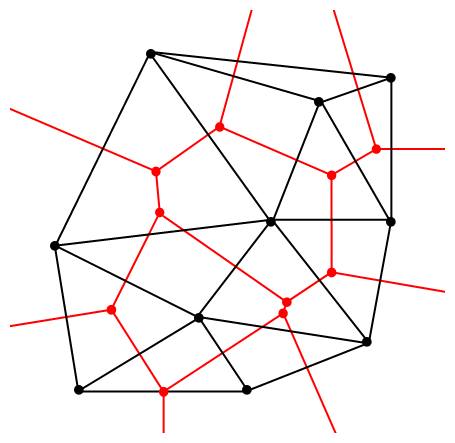
\includegraphics[width=130px]{images/voronoi_delaunay_example_01.png}
\caption{Beispiel einer Delaunay-Triangulation (schwarz) anhand eines Voronoidiagramms (rot)}
\label{fig:delaunayVoronoiExample}
\end{figure}


In der Computergrafik werden in der Regel Polygone verwendet um 2D- oder auch 3D-Modelle darzustellen, sprich, zu rendern. Um diese Modelle möglichst schnell und effizient darzustellen wird bei den Grafikkarten stark auf Optimierung gesetzt. So wird eine Fläche, welche aus Dreiecken besteht, sehr effizient dargestellt. Dies, da ein Dreieck aus drei Punkten besteht und alle diese Punkte auf der selben Ebene liegen, was den Vorgang der Rasterisierung (vereinfacht, die Darstellung einer n-dimensionalen Szene auf einer zweidimensionalen Fläche) deutlich vereinfacht.

Die Delaunay-Triangulation ermöglicht es auf eine effiziente Weise beliebige Flächen zu triangulieren. Wie bereits in~\ref{sec:introduction} erwähnt, kann dies beispielsweise dazu genutzt werden um eine Oberfläche in einem Geoinformationssystem oder ein Polygonnetz zur Darstellung eines dreidimensionalen Modells in einer in Echtzeit auf digitaler Hardware erzeugten multimedialen Präsentation zu erzeugen.

\begin{figure}[h]
\centering
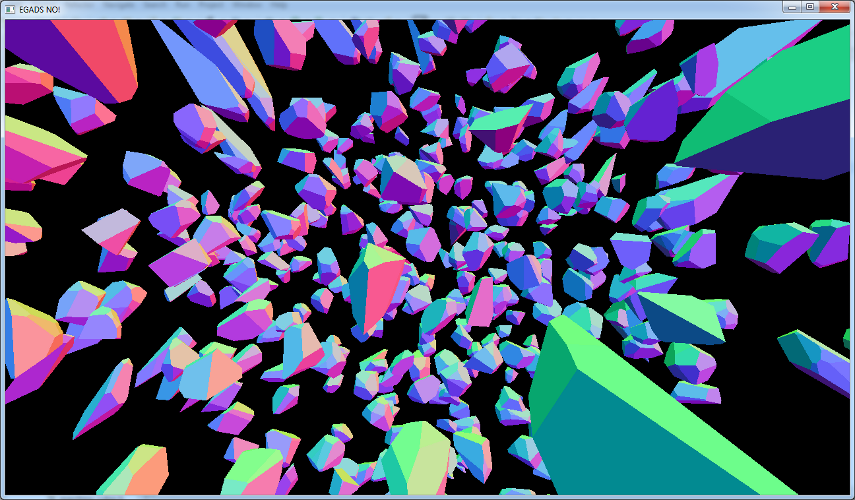
\includegraphics[width=200px]{images/voronoi_delaunay_example_02.png}
\caption[width=100px]{Beispiel von Polygon-Modellen, welche mit Delaunay-Triangulation erzeugt wurden}
\label{fig:delaunayVoronoiExample2}
\end{figure}


\subsection{Definition und Struktur}

Der Einfachheit halber wird in diesem Abschnitt der Raum $\mathbb{R}^2$ anstatt der unter ~\ref{subsec:voronoi-introduction} eingeführte Raum $\mathbb{R}^m$ verwendet.

Die Voronoi-Region $VR(p, O)$ besteht aus allen Punkten der Ebene, denen der Punkt $p = {p_x, p_y}$ näher ist als jeder andere Punkt aus der Punktemenge $O$.

Entfernt man nun sämtliche Voronoi-Regionen aus der Ebene, bleiben genau die Punkte des Raumes $\mathbb{R}^2$ übrig, die keinen eindeutigen sondern zwei oder mehr nächste Nachbaren in der Objekt-Menge $O$ besitzen.

Diese Punktemenge ist das \textit{Voronoi-Diagramm} $V(O)$ von $O$. \parencite{klein2005algorithmischegeometrie}


\subsection{Algorithmen}
\label{sub:delaunayAlgorithms}
Wie in~\ref{sub:voronoiAlgorithms} bereits erwähnt, sind die beiden Strukturen Voronoi-Diagramm $V(S)$ und Delaunay-Triangluation $DT(S)$ dual. Dies heisst, dass sich eine Struktur in der Zeit $O(n)$ aus der anderen Struktur ableiten lässt.

Es wird angenommen, dass das Voronoi-Diagramm $V(S)$ gegeben ist. Man wählt nun eine beliebige Voronoi-Kante zweier Regionen des Diagramms und verbindet nun die Punkte, welche diese Kante erzeugen (Voronoi-Knoten) und erhält so eine Delaunay-Kante. Diese ist senkrecht zu der Voronoi-Kante. Man wiederholt dies für alle Voronoi-Kanten im Voronoi-Diagramm und erhält so ein zweite Tesselation der kovexen Hülle der Voronoi-Knoten.

Ist ein Delaunay-Diagramm ``degeneriert'', ist es u.U. nicht zusammenhängend oder enthält Voronoi-Knoten vom Grad grösser als drei, so handelt es sich nach den oben genannten Schritten nicht um eine Delaunay-Triangluation sondern um eine Delaunay-Pretriangulation. Diese enthält Polygone bestehend aus vier oder mehr Punkten. Diese Polygone lassen sich nun wiederum in Dreiecke unterteilen indem man zwei Eckpunkte so verbindet, dass das entstehende Liniensegment kein anderes schneidet. So erhält man wiederum eine Delaunay-Triangluation.

Es gibt diverse Algorithmen um direkt aus einer Punktemenge eine Delaunay-Triangluation vorzunehmen, es sind dies z.B.

\begin{compactitem}
\item Flip-Verfahren
\item Das Verfahren der inkrementellen Konstruktion
\item Divide-and-Conquer-Verfahren (siehe~\ref{ssub:voronoiAlgorithmsDivAndConq})
\item Sweep (siehe~\ref{ssub:voronoiAlgorithmsSweep})
\end{compactitem}

Diese einzeln vorzustellen und auf deren Laufzeitverhalten und Komplexität zu untersuchen würde den Rahmen dieses Berichtes jedoch sprengen, daher wird darauf verzichtet.


\subsection{Zusammenhang mit Voronoi-Diagrammen}
[Erklärung der Dualität von \\
Voronoi-Diagrammen und der Delaunay-Triangulation.]


\subsection{Praktische Anwendung}
[Ausblick auf praktische Anwendungen und Implementationen, ggf. eigene Implementation.]




\newpage

\section{Schlusswort}
[Zusammenfassendes Schlusswort der Arbeit.]

\newpage

\section{Literaturliste}

\printbibliography

\newpage

\printglossary[numberedsection]

\end{document}
